\chapter{6. State Pattern}
\section{Đặt vấn đề - Máy Gumball}
Ngôn ngữ Java đã và đang trở nên rất thịnh hành ở thời điểm hiện tại. Rất nhiều thiết bị hiện đại có thể xây dựng dựa trên Java. Hãy cùng thử làm một chiếc Máy Gumball!\\[0.1in]
Trong máy Gumball có rất nhiều trạng thái được mô tả thông qua lược đồ dưới đây:

\begin{figure}[!htb]
    \centering
    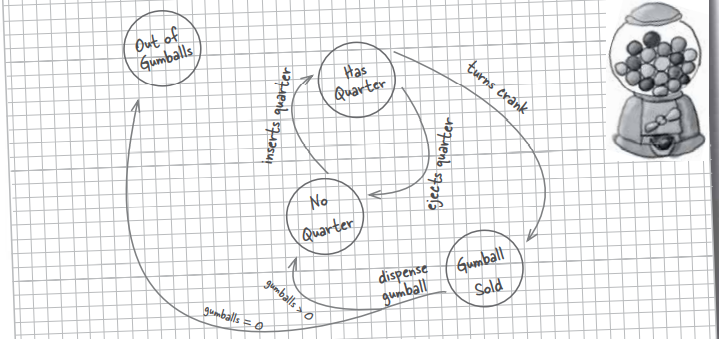
\includegraphics[width=\textwidth]{fig/State/Gumballs_386.png}/
\end{figure}

Bức hình có 4 đường tròn, đó là những trạng thái. \textbf{No Quarter} là trạng thái bắt đầu khi mà trong máy chưa có đồng xu nào. Khi nhét đồng xu vào, nó sẽ chuyển sang trạng thái \textbf{Has Quarter}. Lúc này, ta có thể gạt tay quay để lấy kẹo. Sau đó, máy sẽ kiểm tra lượng kẹo còn lại trong trạng thái \textbf{Gumball Sold} mà quyết định trở về trạng thái \textbf{No Quarter} hay là \textbf{Out of Gumballs}\\[0.1in]

Ta có thể tạo ra lớp \textbf{GumballMachine} như sau:
\begin{itemize}
\item Bước 1: Tập hợp lại các trạng thái:
    \begin{figure}[!htb]
    \centering
    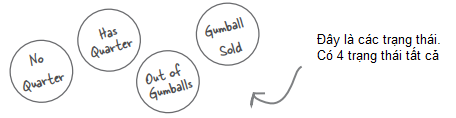
\includegraphics[width=\textwidth]{fig/State/GumballState.png}/
    \end{figure}
\item Bước 2: Tạo các biến static để lưu trạng thái hiện tại và xác định giá trị cho mỗi trạng thái
    \begin{figure}[!htb]
    \centering
    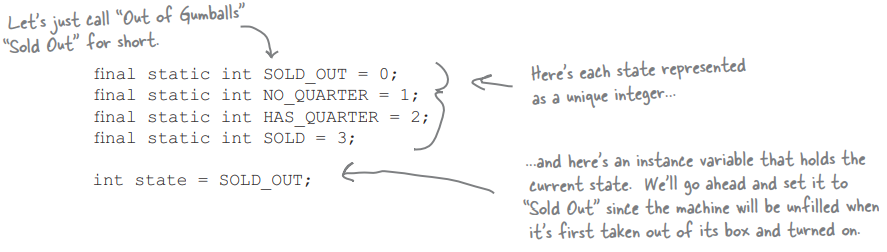
\includegraphics[width=\textwidth]{fig/State/Gumballs_388B2.png}/
    \end{figure}
\item Bước 3: Tập hợp lại những hành động có thể xảy ra trong hệ thống
    \begin{figure}[!htb]
    \centering
    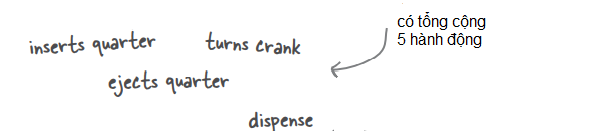
\includegraphics[width=\textwidth]{fig/State/Gumballs_388B3.png}/
    \end{figure}
\item Bước 4: Tạo phương thức ứng với mỗi hành động và sử dụng biểu thức điều kiện để quyết định những hành vi hợp lý ứng với mỗi trạng thái 
\end{itemize}

Dưới đây là code minh họa cho lớp \textbf{GumballMachine}:\newpage

\begin{figure}[!htb]
    \centering
    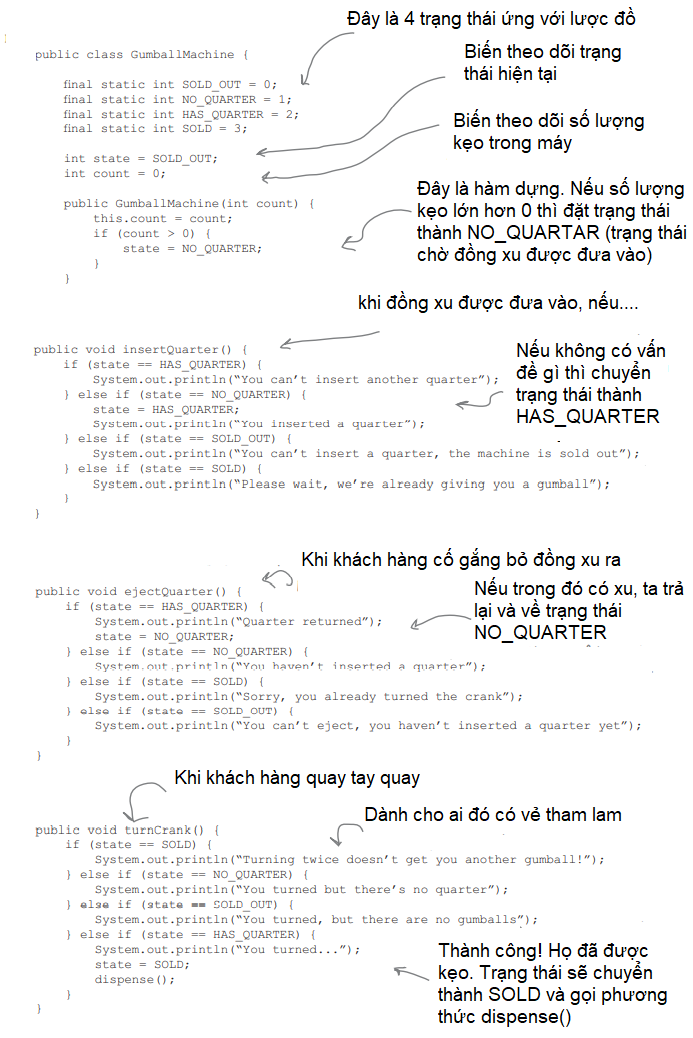
\includegraphics[width=\textwidth]{fig/State/GumballMachine_390.png}/
\end{figure}
\begin{figure}[!htb]
    \centering
    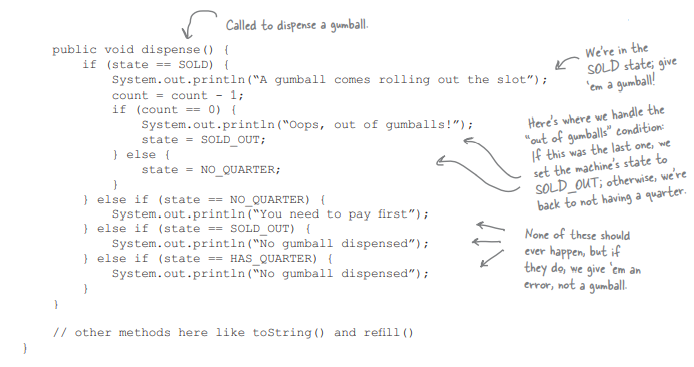
\includegraphics[width=\textwidth]{fig/State/GumballMachine_390_2.png}/
\end{figure}\smallskip

Chương trình ta đã làm rất tuyệt vời nhưng tiếc là đời không như là mơ. Chỉ viết máy Gumball bằng một suy nghĩ thấu đáo như vậy không có nghĩa là nó sẽ dễ dàng phát triển. Giờ khi cải tiến máy với tính năng gấp đôi kẹo nhận được cho người may mắn thì chuyện gì sẽ xảy ra? Khi nghĩ lại đoạn code để nghĩ cách sửa đổi nó thì...
\begin{figure}[!htb]
    \centering
    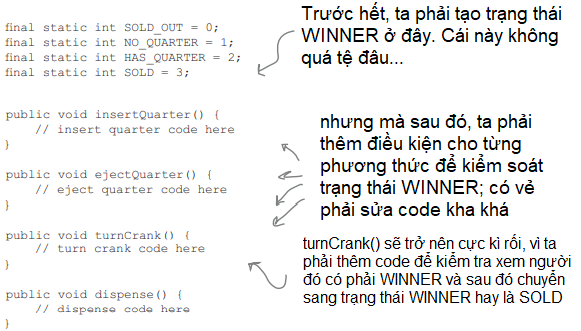
\includegraphics[width=\textwidth]{fig/State/GumballProblem.png}/
\end{figure}\smallskip

\newpage
Vì vấn đề này, ta cần có hướng thiết kế mới. Ta cần cải thiện sao cho code dễ dàng phát triển. Sau đây là cách có thể làm:\smallskip

\begin{itemize}
    \item Trước hết, ta sẽ xác định một \textbf{State Interface} chứa phương thức cho mỗi hành động của máy Gumball
    \item Sau đó, chúng ta bắt đầu cài đặt \textbf{State Class} ứng với mỗi trạng thái của máy. Những lớp này phụ trách cho hành vi của máy khi ở trạng thái tương ứng
    \item Cuối cùng, ta sẽ thay thế biểu thức điều kiện với sự ủy quyền tới những \textbf{State class} để thực hiện công việc
\end{itemize}

Định nghĩa \textbf{State Interface} và các lớp:
\begin{figure}[!htb]
    \centering
    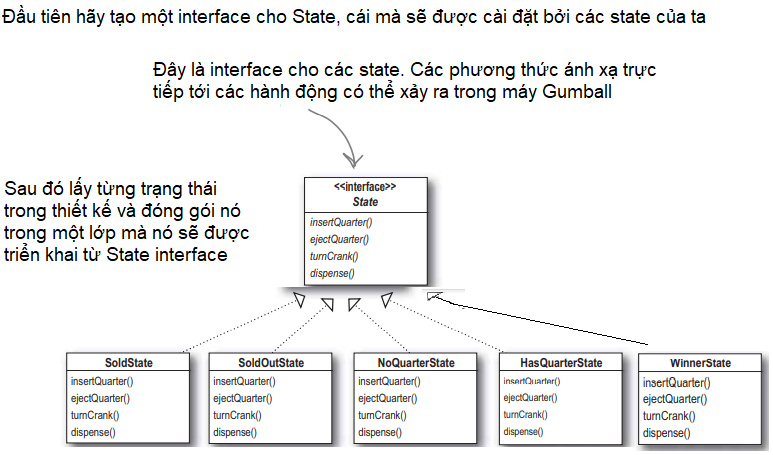
\includegraphics[width=\textwidth]{fig/State/GumballDiagram.png}/
\end{figure}\newpage

Sau đó, tiến hành cài đặt các lớp của \textbf{State}. Bắt đầu với \textbf{NoQuarterState}:
\begin{figure}[!htb]
    \centering
    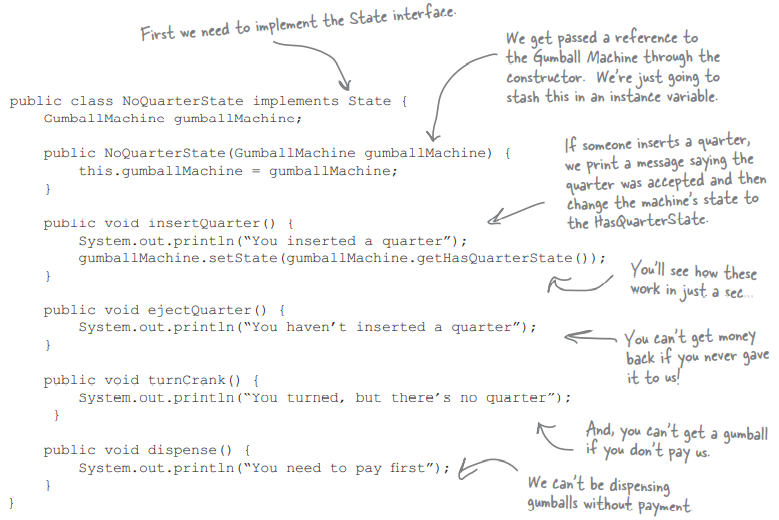
\includegraphics[width=\textwidth]{fig/State/NoQuarterState.png}/
\end{figure}\smallskip

Tiếp theo là \textbf{HasQuarterState} và \textbf{SoldState}:

\begin{figure}[!htb]
    \centering
    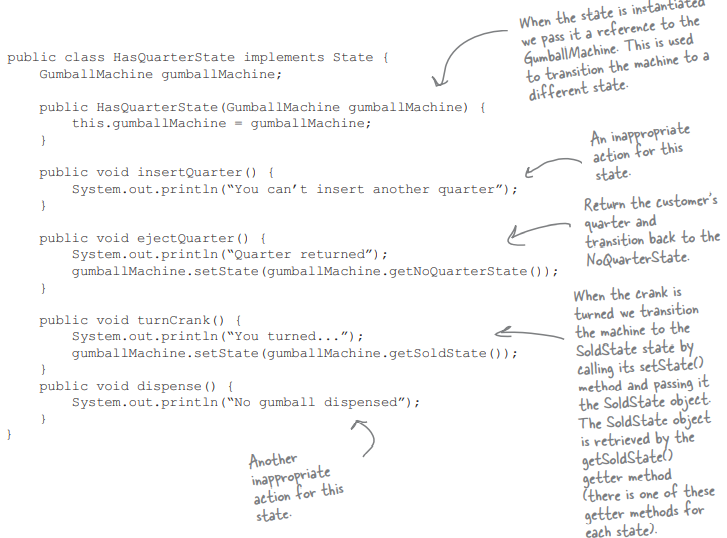
\includegraphics[width=\textwidth]{fig/State/HasQuarterState.png}/
\end{figure}\bigskip

\begin{figure}[!htb]
    \centering
    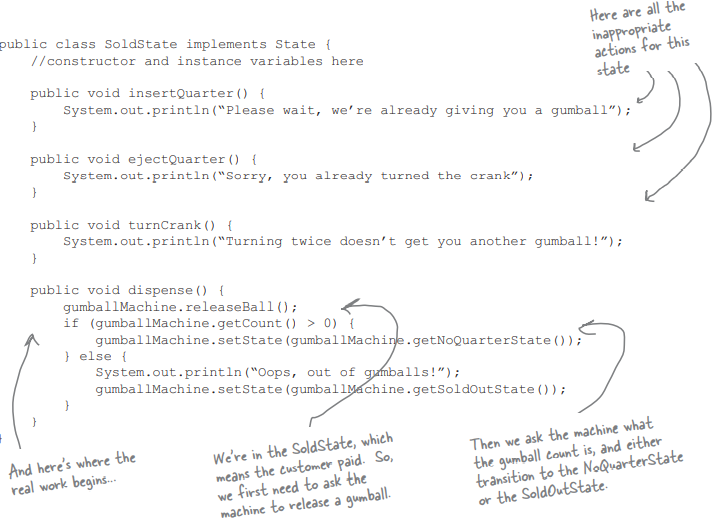
\includegraphics[width=\textwidth]{fig/State/SoldState.png}/
\end{figure}\newpage

Tương tự với 2 \textbf{SoldOutState} và \textbf{WinnerState}. Cuối cùng là lóp \textbf{GumballMachine} hoàn chỉnh:

\begin{figure}[!htb]
    \centering
    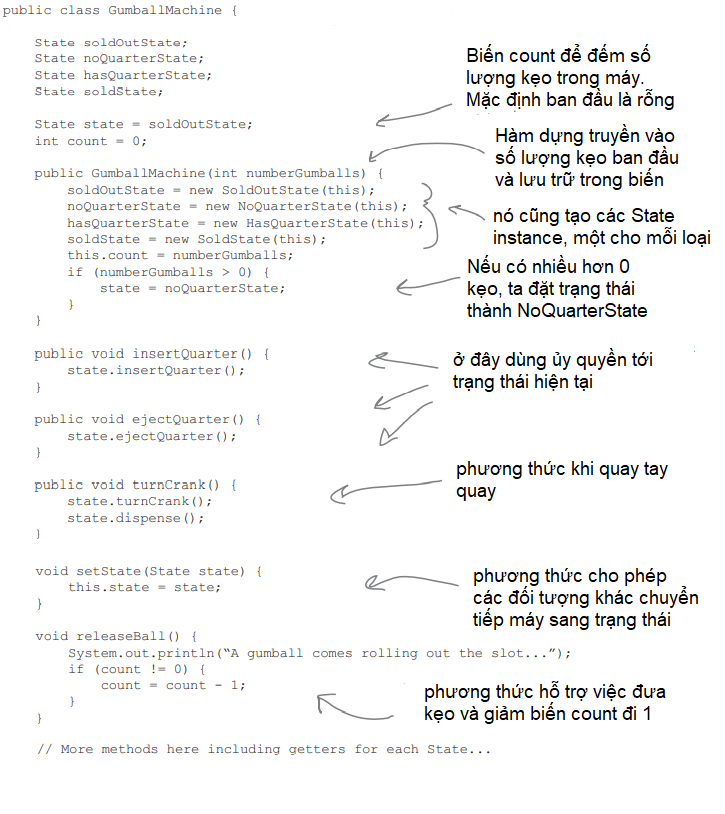
\includegraphics[width=\textwidth]{fig/State/GumballMachine_code.png}/
\end{figure}

Nhìn lại những gì trước đó đã làm, ta đã thay đổi cấu trúc khác biệt so với bản đầu tiên nhưng chức năng vẫn không đổi. Cách thiết kế này có tên gọi là \textbf{State Pattern} Bằng cách này, ta đã:

\begin{itemize}
    \item Tách biệt hành vi của từng trạng thái đến từng lớp
    \item Loại bỏ tất cả biểu thức điều kiện rắc rối gây khó khăn trong việc bảo trì
    \item Đóng từng trạng thái cho việc sửa đổi nhưng vẫn để Máy Gumball được phát triển bằng cách thêm mới nhiều lớp trạng thái
    \item Tạo một code base và cấu trúc lớp ánh xạ tương đồng tới bản thiết kế ban đầu, dễ đọc, dễ hiểu
\end{itemize}

\section{Định nghĩa và Mô hình cấu trúc}
\subsection{Định nghĩa}
\textbf{State Pattern} cho phép một đối tượng thay đổi hành vi của nó khi trạng thái bên trong thay đổi. Đối tượng sẽ xuất hiện để thay đổi lớp của nó
\subsection{Mô hình cấu trúc}
Dưới đây là mô hình cấu trúc của \textbf{State Pattern}:
\begin{figure}[!htb]
    \centering
    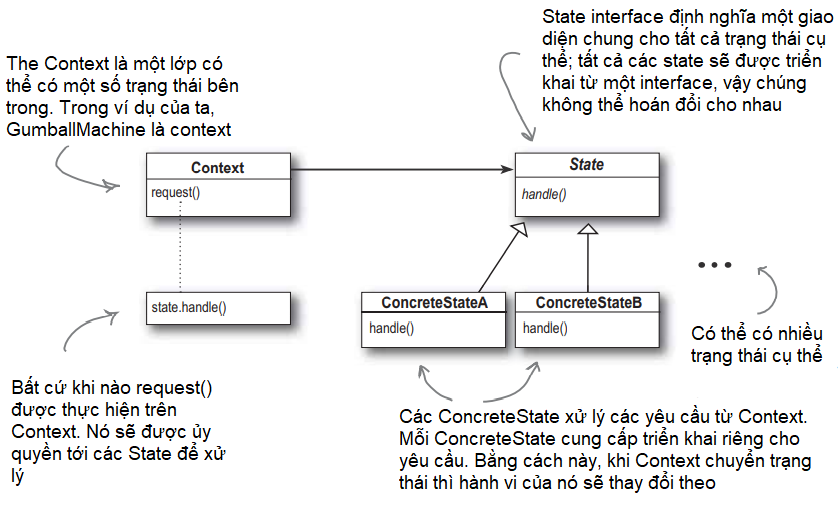
\includegraphics[width=\textwidth]{fig/State/StateDiagram.png}/
\end{figure}

\section{Thực tế}
Johnson and Zweig [JZ91] biểu thị State pattern và ứng dụng tới giao thức kết nối TCP\\[0.1in]
Hầu hết các chương trình vẽ phổ biến đều cung cấp "công cụ" để thực hiện các thao tác trực tiếp. Ví dụ: một công cụ vẽ đoạn thẳng cho phép người dùng nhấp và kéo để tạo một đường mới. Một công cụ lựa chọn cho phép người dùng chọn các hình khối. Thường có một bảng các công cụ để lựa chọn. Người dùng coi việc này này như nhặt một dụng cụ và sử dụng nó, nhưng trên thực tế, hành vi của editor thay đổi với công cụ hiện tại: Khi một công cụ vẽ hoạt động, ta tạo ra các hình khối; khi mà
công cụ lựa chọn đang hoạt động ,ta chọn các hình khối đó; và cứ thế. Ta sử dụng State pattern để thay đổi hành vi của editor tùy thuộc vào công cụ hiện tại.\\[0.1in]
Ta có thể định nghĩa lớp trừu tượng Tool để từ đó định nghĩa các lớp con mà cài đặt các hành vi cụ thể. Trình chỉnh sửa bản vẽ duy trì một đối tượng Tool và ủy quyền các yêu cầu tới nó. Trình sẽ thay thế đối tượng khi người dùng chọn công cụ mới khiến hành vi của trình vẽ thay đổi theo\\[0.1in]
Kĩ thuật này được áp dụng dụng trong những framework hỗ trợ chỉnh sửa bản vẽ điển hình như HotDraw [Joh92] và Unidraw [VL90]. Nó cho phép phía Client định nghĩa nhiều loại công cụ một cách dễ dàng. Trong HotDraw, lớp DrawingController chuyển tiếp các yêu cầu đến đối tượng Tool hiện tại. Còn Unidraw sẽ có lớp tương ứng là Viewer và Tool. Dưới đây là mô hình cấu trúc cho Tool và DrawingController interfaces:
\begin{figure}[!htb]
    \centering
    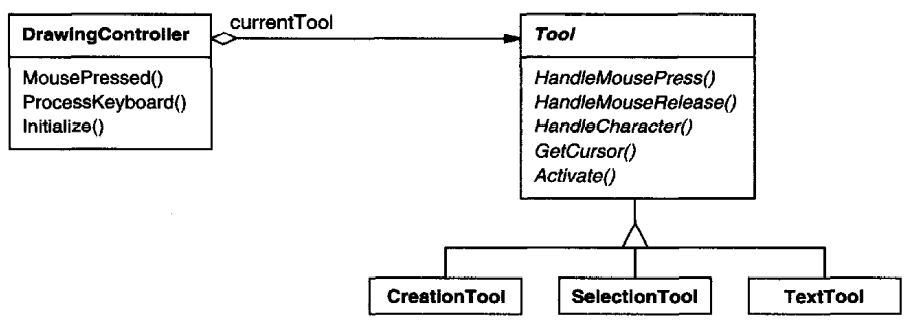
\includegraphics[width=\textwidth]{fig/State/StateRealLifeEX.png}/
\end{figure}